\chapter{Structure du code}

Maintenant que les besoins ont étés traîtés, il convient de s'intéresser à la façon dont nous allons organiser notre code. 
Puisque nous avons choisi Java comme langage de programmation, la conception du programme se fera sous la lumière de la programmation orientée objet. 
Il faut donc définir les classes qui seront utilisées dans le projet.

\paragraph{Le Rubik's cube} Premièrement, notre programme manipule un Rubik's cube. 
Il s'agit donc de définir l'organisation de ces objets:

\begin{figure}[h]
\begin{center}
      \makebox[\textwidth]{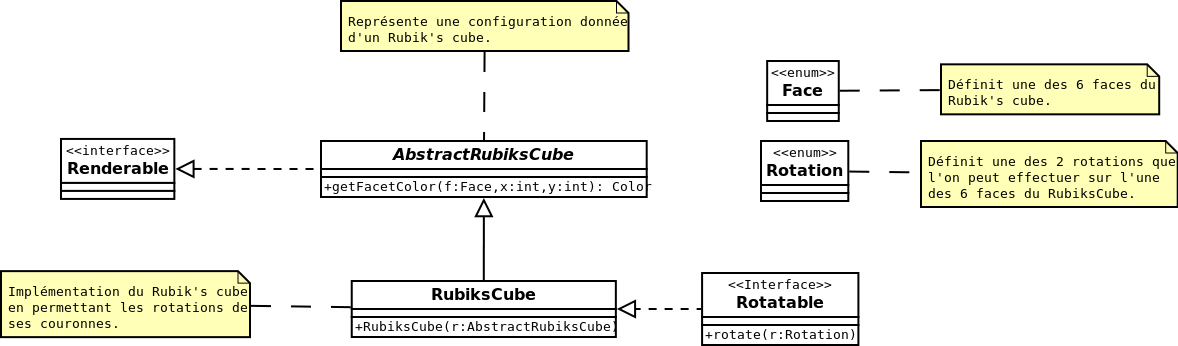
\includegraphics[width=.8\paperwidth]{diagrammes/rubikscube.png}}
\end{center}
    \caption{Diagramme des classes modélisant le Rubik's Cube}
\end{figure}

Ainsi \textit{AbstractRubiksCube} servira lorsque que nous aurons besoin d'informations sur une configuration donnée du Rubik's Cube alors que \textit{RubiksCube} permettra la manipulation de cet objet via l'interface \textit{Rotatable}. 


\paragraph{Rubik'Int} Notre application - donc notre classe principale - sera appelée RubikInt. Elle aura pour rôle de commander les autres objets pour que le programme ait le comportement désiré. Ainsi on peut dessiner un diagramme montrant ses interactions avec les différents autres objets (voir ci-dessous).

\begin{figure}[h]
\begin{center}
      \makebox[\textwidth]{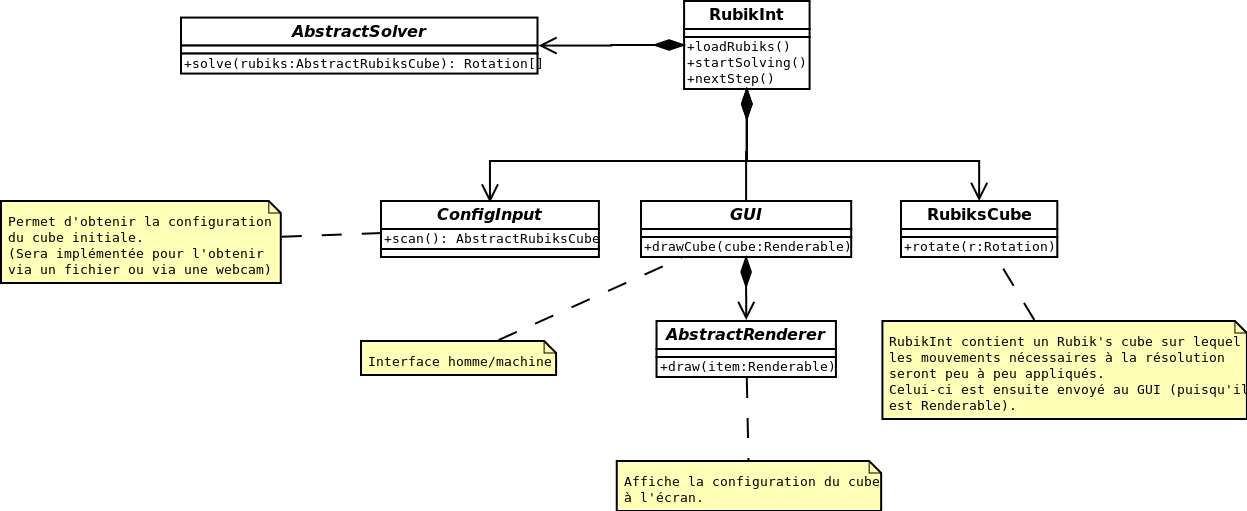
\includegraphics[width=.8\paperwidth]{diagrammes/projet.png}}
\end{center}
    \caption{Diagramme des classes du projet}
\end{figure}

On voit sur le diagramme les différents point importants de notre projet. 
\begin{itemize}
    \item L'interface homme/machine, qui se caractérise par l'implémentation de des classes filles de \textit{GUI} et \textit{AbstractRenderer}.
    \item L'algorithme de résolution qui devra être mis en place dans l'implémentation de la classe fille de \textit{AbstractSolver}. Plusieurs variantes pourront êtres mises en oeuvre.
    \item La structure de donnée choisie pour représenter le Rubik's Cube, dans sa classe \textit{RubiksCube}.
    \item L'interface permettant de rentrer la configuration d'un Rubik's Cube dans \textit{ConfigInput}. Nous pourrons par exemple charger cette configuration d'un fichier, laisser l'utilisateur la rentrer sur une interface graphique ou même l'obtenir via une caméra.
\end{itemize}


